\chapter{Muon Telescope Detector}

A large-area, cost-effective Muon Telescope Detector (MTD) at mid-rapidity for the STAR can trigger on and identify muons based on its precise timing and modest position resolution, allowing us to measure dilepton through di-$\mu$ channel. Compared with electrons, muons have less background from gamma conversions and suffer less bremsstrahlung radiation energy loss effects in the detector materials. These make the muon be a more effective triggering particle in central nucleus-nucleus collisions at mid-rapidity at the STAR. The novel and compact device allows for the measurements of quarkonia, dilepton continuum (di-$\mu$ channel), as well as the correlation of heavy flavor quarks through their semi-leptonic decays (e-$\mu$ channel). The di-$\mu$ channel can be used to measure the J/$\psi$ meson over a broad transverse momentum range thanks to the low kinematic threshold of the MTD trigger on muons. It also has the potential to separate different $\varUpsilon$ states, predicted to melt at very different temperatures, as the bremsstrahlung radiation for muons is much smaller compared to electrons. The e-$\mu$ correlation can be used to distinguish between lepton pair production and heavy quark decays ($c + \overline{c} \rightarrow e + \mu(e), B \rightarrow e(\mu) + c \rightarrow e + \mu(e)$), allowing us directly access the QGP thermal radiation. The MTD will thus provide direct information on the temperature and the characteristics of color screening in the QGP created in RHIC collisions.

\section{MTD Configuration}

Out of the full MTD system, 10\%  (12 modules), 61\% (75 modules) and 100\% (122 modules) were installed in years 2012, 2013, 2014, respectively. The whole MTD system, covering $|\eta|$ < 0.5 and 2$\pi$ azimuthal, is mounted on BEMC PMT boxes behind the STAR magnet flux-return bars so called ``backlegs'' which serve as hadron absorbers. The schematic and physical picture are shown in Fig.~\ref{mtdsys}. There are 30 backlegs outside the magnetic coils to provide the return flux path for the magnetic field~\cite{STARmagnet} with only 28 of them mounted with MTD trays due to the mechanical constraints. Each backleg covers 8$^{\circ}$ in azimuthal while the gap between two backlegs covers 4$^{\circ}$. Nineteen of 28 MTD trays are five-module trays while two (BL8, BL24) of them are not fully shielded by the magnetic steels. Thus 3 $\times$ 5, 2 $\times$ 5 readout channels (exposed in the backleg gap) are disabled for BL8 and BL24, respectively, avoiding hot channels in the MTD trigger system. The remaining 9 bottom MTD trays are three-module trays due to the two cradles. Figure~\ref{mtdhitmap} shows the hit map of the MTD system during the run15 $p$ + $p$ at $\sqrt{s_{NN}}$ = 200 GeV.

\begin{figure}
\centering
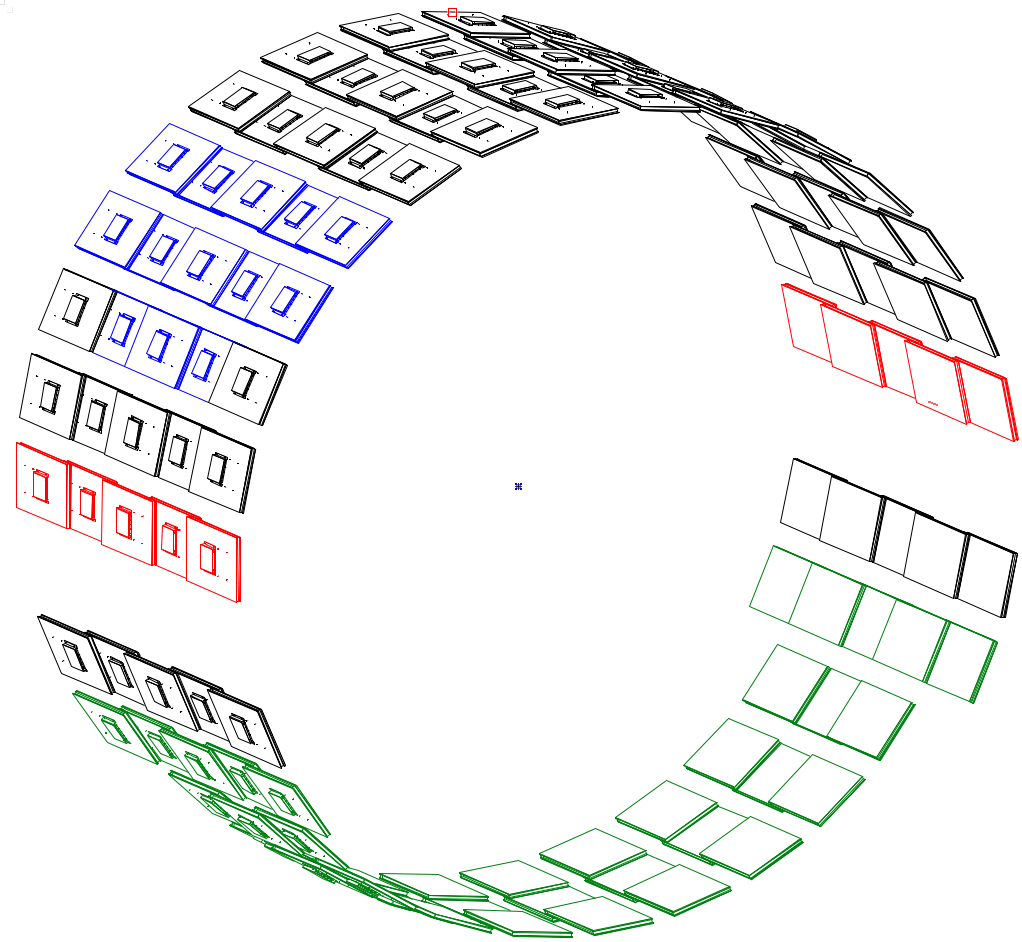
\includegraphics[width=0.48\textwidth]{mtd/MTD_schematics.png}
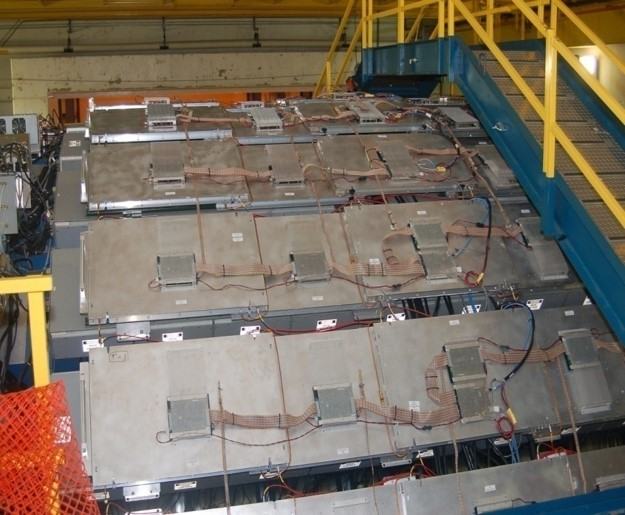
\includegraphics[width=0.48\textwidth]{mtd/MTD_reality.jpg}
\figcaption{(Left) The schematic view of the whole MTD system. Different colors represent the modules installed in different years: Blue - installed in year 2012; Black - installed in year 2013; Green and Red - installed in 2014, the two red trays are special trays with 2$\times$5 (in BL24) and 3$\times$5 (in BL8) readout channels disabled. (Right) The physical picture of the MTD system.}
\label{mtdsys}
\end{figure}

\begin{figure}[htbp]
\centering
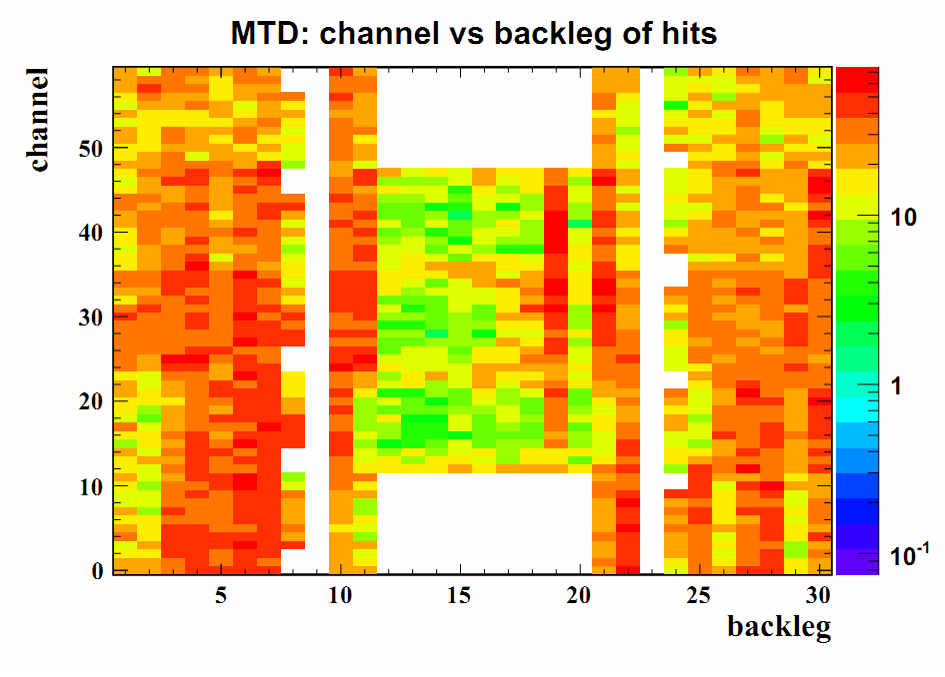
\includegraphics[keepaspectratio,width=0.7\textwidth]{mtd/MTDHitMap_pp200.png}
\vspace*{-5mm}
\figcaption{The hit map of the MTD system in the run15 $p$ + $p$ at $\sqrt{s_{NN}}$ = 200 GeV.}
 \label{mtdhitmap}
\end{figure}

The MTD detector is based on large Multi-gap Resistive Plate Chambers with long readout strips (LMRPC)~\cite{MTDdet}. Couple of prototypes with different designs were tested at T963 at Fermilab and beam line 3 at Institute of High Energy Physics (IHEP), resulting in $<$70 ps timing resolution and $\sim$1 cm spatial resolution along the readout strip with $>$95\% detection efficiency~\cite{MTDmrpc0,MTDmrpc1}. The final design of the LMRPC module is shown is Fig.~\ref{mtdmrpc}. The module has five 250 $\mu$m gas gaps which are defined by a stack of float glass sheets separated by a nylon monofilament fishing line. The thickness of the float glass (inner glass) sheets is 0.7 mm while the volume resistivity is $\sim$10$^{13}$ $\Omega\cdot$cm. The positive and the negative high voltage (HV) are applied to a coating of colloidal graphite paint (with surface resistivity of 1$\sim$10 M$\Omega$/$\Box$) on the external surface of the outer glass plates. The 3-D size of the outer glass is 890 $\times$ 559 $\times$ 1.1 mm$^{3}$. The total area of each LMRPC module defined by the Printed Circuit Board (PCB) is 915 $\times$ 580 mm$^{2}$ while the active area defined by the inner glass sheets is 874 $\times$ 543 mm$^{2}$. Twelve double-end readout strips are fixed on the PCB facing inner glasses, and the size of each strip is 870 mm long and 38 mm wide. The width of the intervals between two readout strips is 6 mm. Two pieces of 10 mm thick honeycomb-board are attached to the outer surfaces of the detector to reduce structural deformations.

\begin{figure}[htbp]
\centering
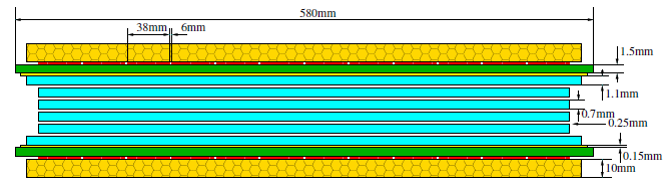
\includegraphics[keepaspectratio,width=1\textwidth]{mtd/MTDmrpc.png}
\figcaption{A schematic side-view of the LMRPC module.}
 \label{mtdmrpc}
\end{figure}

\begin{figure}[htbp]
\centering
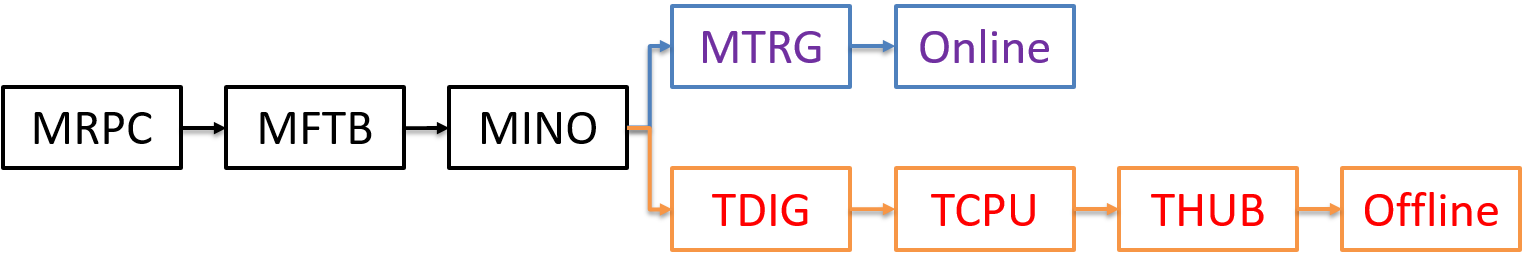
\includegraphics[keepaspectratio,width=1\textwidth]{mtd/MTDelectronics.png}
\figcaption{A schematic view of the MTD electronics and readout paths.}
 \label{mtdelectronics}
\end{figure}

The signals from the LMRPC modules are digitized by two different sets of electronics, shown in Fig.~\ref{mtdelectronics}, while the electronics for precise timing measurements is the same as that for the STAR TOF~\cite{TOFelectronics}. The signals from the MTD are sent to a MINO board to perform a leading-edge discrimination through a MFTB board. The outputs of the MINO board are sent to a TDIG board which uses the CERN HPTDC chip~\cite{HPTDC} to digitize the arrival times of the signals with respect to an externally input free-running 40 MHz clock. Each TDIG board uses three HPTDC chips in ``high resolution'' mode. The digitized times are 21 bit data words with a dynamic range of 52 $\mu$s and the least significant bit (LSB) time conversion is 25 ns/1024 $\approx$24.4 ps. The magnitude of the MTD signals is characterized by the width of output digital signals from MINO board called ``Time Over Threshold'' (TOT). A copy of  MINO outputs is passed to a MTRG board through a MTRG cable and combined with a logical "OR". Then, the outputs of the MTRG board are sent to electronics in the STAR trigger system called ``QT boards'' through long coax cables. The QT board performs magnitude and timing measurements using an analog-to-digital (ADC) and timing-to-amplitude (TAC) circuitry. The ADC and TAC measurements are each 12-bit numbers while the TAC timing measurement uses a common stop with respect to the 9.4 MHz RHIC clock with a digital-to-time conversion of $\sim$18 ps/LSB. The trigger logic of the MTD system will be discussed in details in Sec.~\ref{mtdtriggersection}. 

\section{MTD Trigger Logic}
\label{mtdtriggersection}

The whole MTD system (122 MTD modules) is divided into 28 MTD trigger patches. In general, one trigger patch is composed of 5 MTD modules in the same $\eta$ region. The same $\eta$ guarantees that the path lengths from collision vertex to the MTD modules of the same trigger patch are the same. Due to the asymmetric MTD geometry in $\phi$ direction, there are some trigger patches composed of less than 5 MTD modules. The signals from the MTD trigger patches are sent to QT boards (first layer of trigger system) numbered MT001 - MT004. The detail trigger patch compositions and the logic from trigger patches to QT boards can be found in Fig.~\ref{mtdtrgflow} and App.~\ref{chap:mtdtrgmap}. A timing cut is applied in the QT board to reject the noise. For each QT board, two earliest hit signals (with largest TAC sum - the read-out strips of MTD module are double-ended) are selected and sent to the next layer of the trigger system (MT101). Then all eight signals in MT101 are compared to the VPD time, and an online timing window is applied to reject the background and slow hadrons. The results of the selection are sent to the third layer of the trigger system called TF201, resulting in a 8-bit sequence. At last, the MTD related bits are formed in the Trigger Control Unit (TCU) based on the 8-bit sequence in TF201. The MTD related triggers generated by combining the bits from the MTD and other detectors (VPD, ZDC etc.), trigger on the interested collision events. The trigger flow of the MTD system for Run14 and Run15 is shown in Fig.~\ref{mtdtrgflow}. 

\begin{figure}[htbp]
\centering
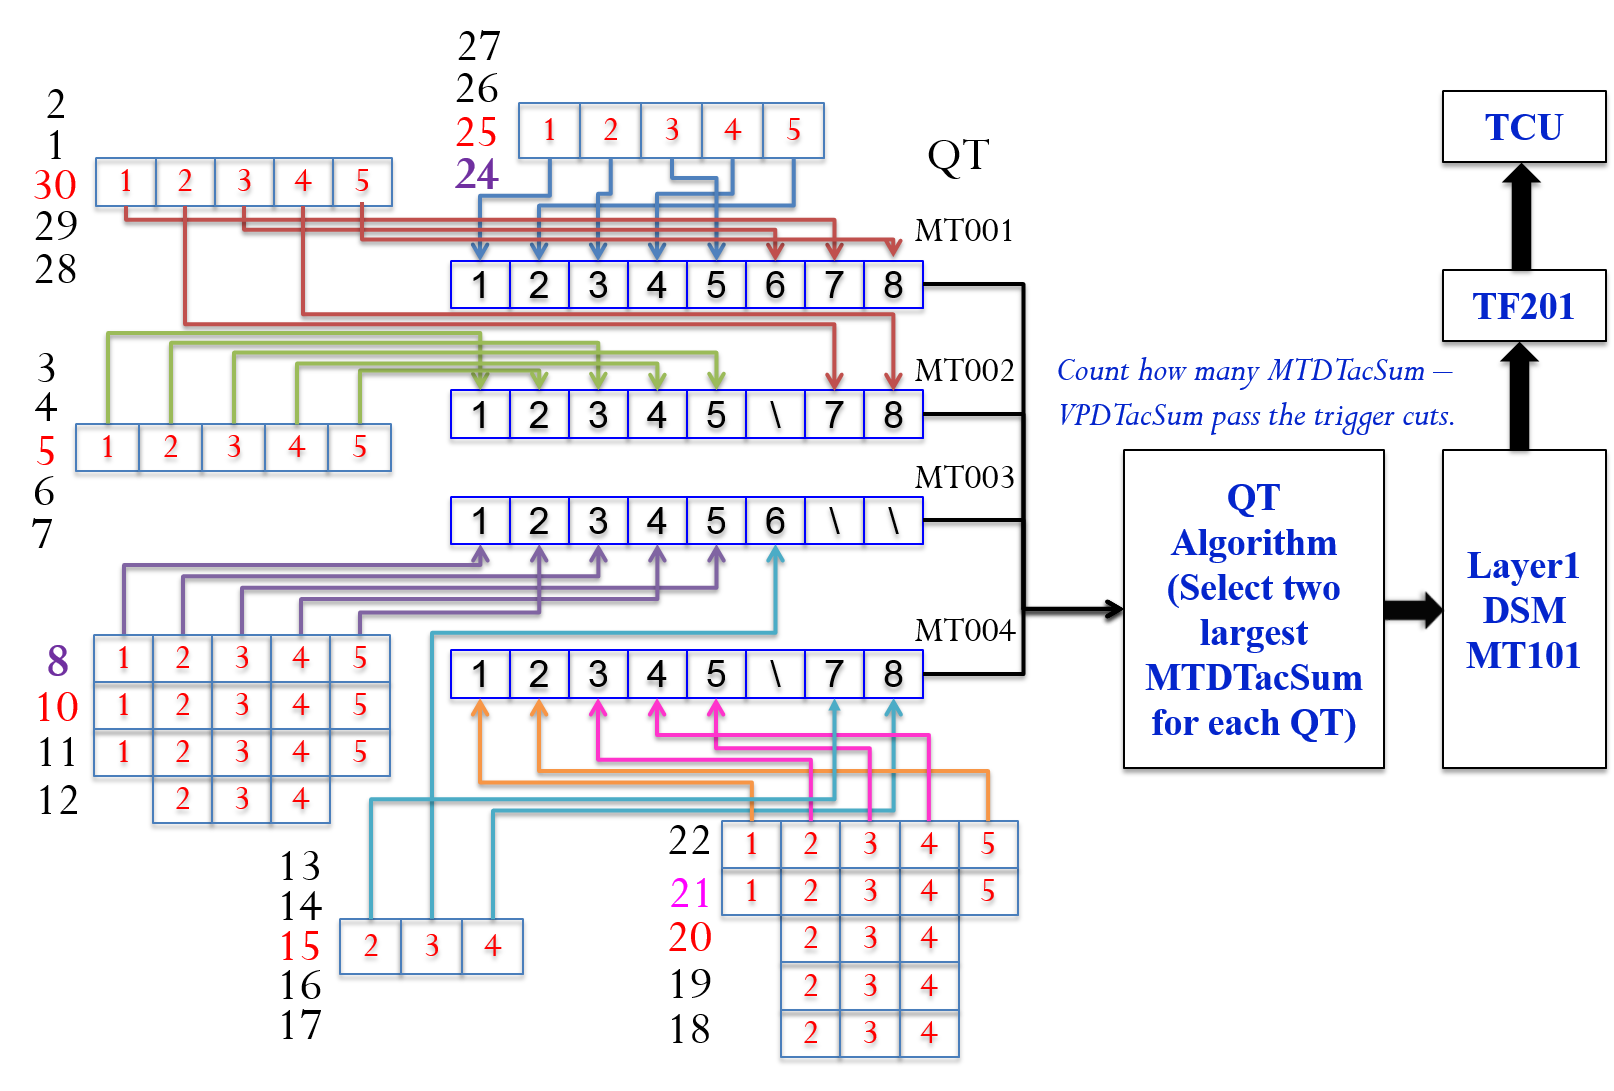
\includegraphics[keepaspectratio,width=1\textwidth]{mtd/mtd_trigger_flow.png}
\figcaption{The trigger flow of the MTD system in Run14 and Run15. In general, one trigger patch consists of 5 MTD modules (e.g. BL28-1, BL29-1, BL30-1, BL1-1, and BL2-1 form a trigger patch). Due to the asymmetric MTD geometry, there are some trigger patches consist of $<$ 5 MTD modules (e.g BL21-1 and BL22-1 form a trigger patch). The \textcolor{red}{\textbf{red}} backleg IDs represent that these backlegs are mounted with MTRG boards. Beside these backlegs, Module 1 and 5 of  BL21 (\textcolor{magenta}{\textbf{magenta}}) are also mounted with MTRG boards. BL8 and BL24 (\textcolor{violet}{\textbf{violet}}) are two special backlegs with 3 $\times$ 5 and 2 $\times$ 5 readout strips disabled, respectively.}
 \label{mtdtrgflow}
\end{figure}

\subsection{QT Algorithm}
The QT algorithm outputs two largest TAC pair sums (two earliest signal pairs from two trigger patches) with an 2-bit ID for each TAC pair sum. The 2-bit ID can tell which TPC sectors are covered by the corresponding trigger patch for partial tracking or ``DAQ 10K'' purpose. ``DAQ 10K'' is a sparse readout scheme for the TPC that would enable STAR to acquire events at rates of 10 kHz for classes of physics where only few TPC sectors contain all the necessary particle information. Each QT board has 32 inputs in a line and the inputs can be numbered 1 - 32 from top to bottom. Each MTD trigger patch has an East-end and West-end readout (mark East-end as $J2$, West-end as $J3$ for the modules located in positions 1, 2, and 3; mark West-end as $J2$, East-end as $J3$ for the modules located in positions 4 and 5) while each end readout occupies two QT input channels recording the magnitude and timing information.

In the QT board, an alignment is applied to each TAC channel, at the very beginning, to eliminate the differences of flight time from collision vertex to MTD tirgger patches due to different path lengths and electronics, shown in Fig.~\ref{tacalignment}. Second, a slewing correction is applied to each TAC channel based on the value of the corresponding ADC channel. After the TAC value modification, the TAC value is filtered by ``Good Hit'' criteria which requires the TAC value for a channel is greater than ``TAC\_Min'' and less than ``TAC\_Max'', to reject noise hits. Both of the $J2$ and $J3$ TAC values from the same trigger patch must satisfy the ``Good Hit'' requirement, otherwise, the TAC sum (TAC$_{sum}$ = TAC$_{J2}$ + TAC$_{J3}$) is set to 0 for this trigger patch. And then, the hit position correction for each trigger patch is applied according to the TAC difference between East-end and West-end TAC (TAC$_{J2}$ - TAC$_{J3}$) to eliminate the influence of different path lengths caused by different hit positions in the same trigger patch along $z$ direction (along beam axis), especially for the outermost trigger patches. The 13-bit corrected TAC pair sum is then truncated to 10 bits. Bits [3:12] (starting from zero) are kept. The two largest truncated, corrected TAC pair sums together with the corresponding 2-bit IDs are then found and transfered to the next layer of the trigger system (MT101).

\begin{figure}
\centering
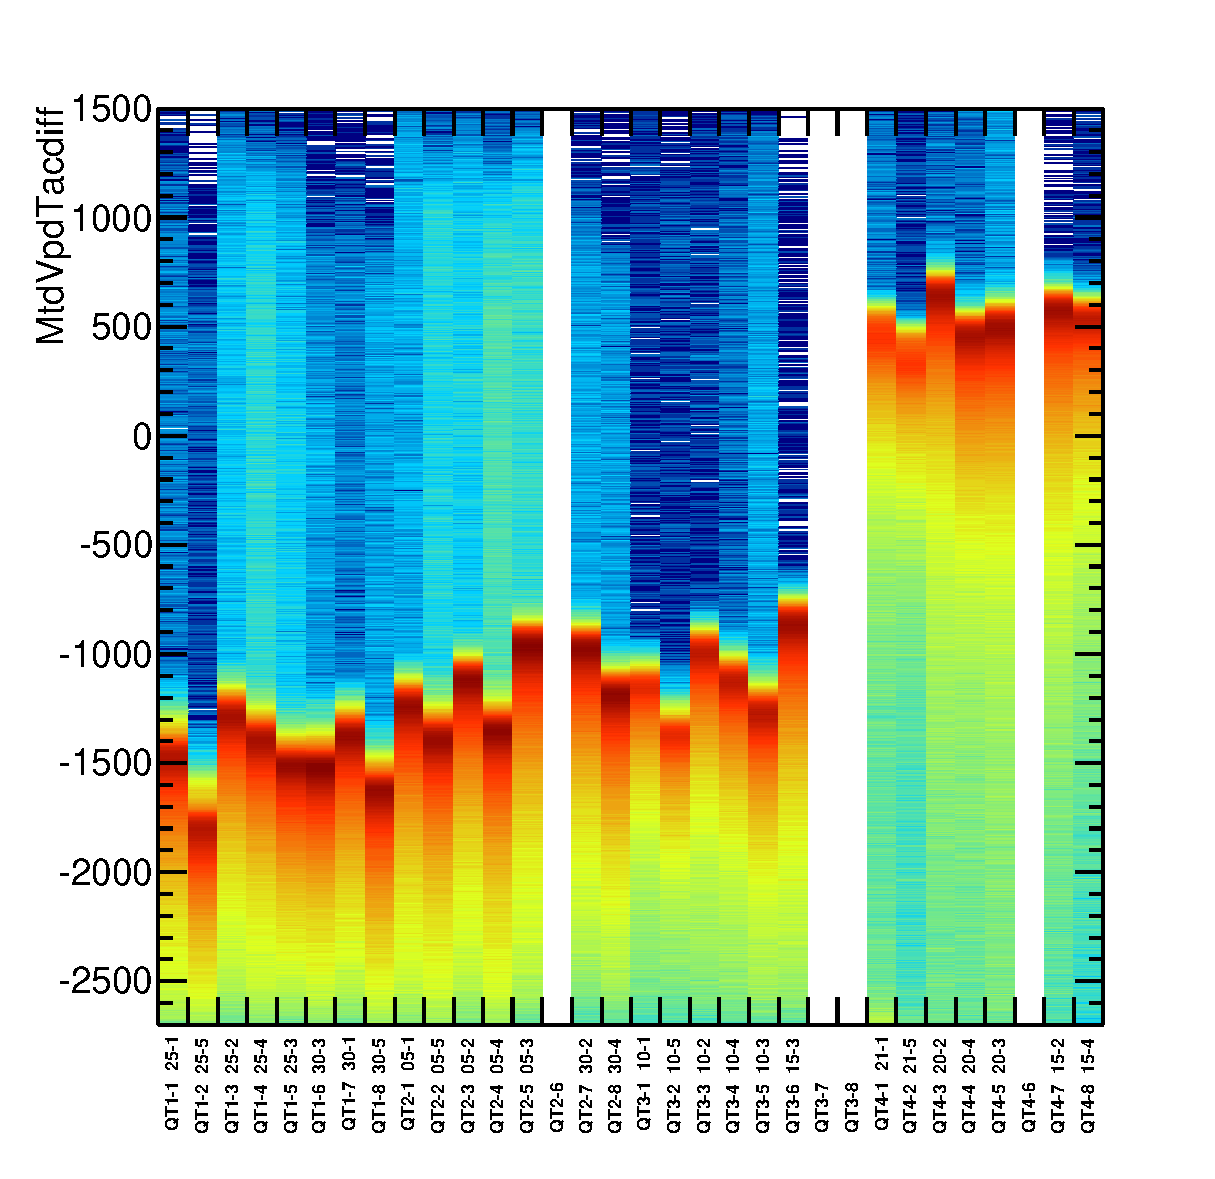
\includegraphics[width=0.48\textwidth]{mtd/MtdVpdTacdiffRawvsQtChannel.eps}
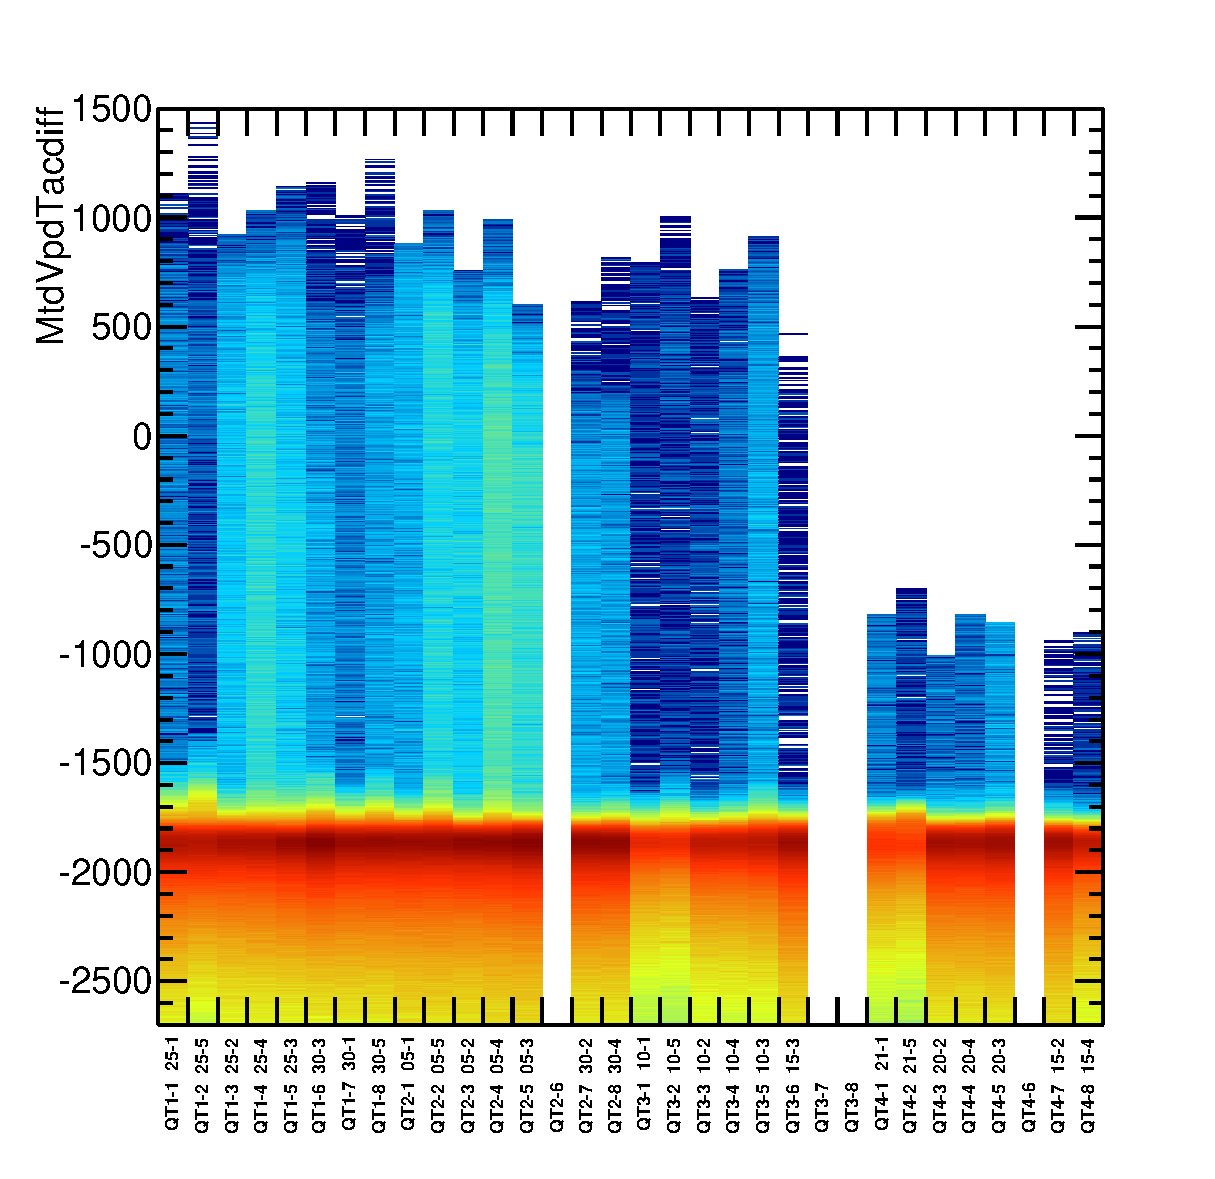
\includegraphics[width=0.48\textwidth]{mtd/MtdVpdTacdiffCorvsQtChannel.eps}
\figcaption{(Left) ``MTD TAC sum - VPD TAC sum'' vs. trigger patch before the TAC alignment in Run 14 Au + Au at $\sqrt{s_{NN}}$ = 200 GeV. (Right) ``MTD TAC sum - VPD TAC sum'' vs. trigger patch after the TAC alignment in Run 14 Au + Au at $\sqrt{s_{NN}}$ = 200 GeV.}
\label{tacalignment}
\end{figure}

\subsection{DSM Algorithm (MT101$\rightarrow$TF201$\rightarrow$TCU)}
The MT101 DSM receives its data through a TDSMI, so there are 10 12-bit input channels. The algorithm receives the 2 best TAC sums from each of the 4 MTD QT boards, and the IDs of those sums. It also receives the fastest (largest) TAC values from the QT boards covering the East and West sides of the VPD. The VPD TAC sum is calculated and truncated from 13 bits to 10 bits. Bits [3:12] (starting from zero) are kept. Then the algorithm finds the difference between the MTD and VPD TAC sums. All 8 MTD VPD TAC differences (MTD\_TAC\_Sum - VPD\_TAC\_Sum + 1024, to guarantee the MTD VPD TAC difference is larger than zero) are checked to determine if they are inside a timing window. If either TAC from East side of VPD, or TAC from West side of VPD, or MTD TAC sum is $\leq$0, the corresponding MTD VPD TAC difference is directly set to zero. Those that are inside the window are counted, and the count is sent to TF201. Meanwhile a 8-bit sequence (``MTD-VPD TAC difference in window'' bits) is sent to TF201 for indicating that each MTD VPD TAC difference is inside the timing window or not (``1'' is inside the window, ``0'' is outside the window). The MTD VPD TAC differences are also sorted to find the two largest values that are inside the window. The 2-bit IDs of those two channels are sent on to MT201 for the DAQ10k readout scheme. In addition, a bit is set if at least two of the incoming MTD TAC sums is non-zero. That bit is sent to TF201 for use as a debugging and monitoring trigger, or for triggering on cosmic rays. The MTD related bits in TCU is formed based on the information stored in TF201. Di-muon bit is set to TRUE if the count of MTD VPD TAC difference inside the timing window is $\geq$2, otherwise set to FALSE. Single-muon bit is set to TRUE if the count is $\geq$1 while MTD-Cosmic bit is set to TRUE if at least two of the MT101 incoming MTD TAC sums are non-zero. The MTD related triggers (di-muon, single-muon, e-muon, mtd-cosmic-ray) are formed based on the combination of TCU bits from the MTD detector and other relevant detectors. Table~\ref{mtdsampledlum} shows luminosity and statistics sampled by the MTD detector in physics Run13, Run14 and Run15. The MTD muon trigger efficiency for the Run14 Au + Au at $\sqrt{s_{NN}}$ = 200 GeV (Centrality: 0-60\%) is shown in Fig.~\ref{muontrgeff}. The overall muon trigger efficiency caused by trigger electronics and algorithm is around 78\%.

\begin{table}[htp]
\centering
\caption{The luminosity and statistics sampled by the MTD related triggers. ``single-muon'' trigger has at least one online muon candidate (provided by the MTD and VPD) and 5 cm online vertex cut (provided by the VPD). ``di-muon'' trigger has at least two online muon candidates and no online vertex cut. ``di-muon-5-hft'' trigger has at least two online muon candidates, 5 cm online vertex cut and read out HFT information. ``di-muon-30-hft'' trigger has at least two online muon candidates, 30 cm online vertex cut and read out HFT information. ``e-muon'' trigger has at least one online muon candidate, one online electron candidate (provided by the BEMC) and 30 cm online vertex cut.}
\label{mtdsampledlum}
\newcolumntype{V}{!{\vrule width 1.6pt}}
\begin{tabular}{Vc|c|c|r@{.}l|r@{.}lV}
\Xhline{1.6pt}
\textbf{Year} & \textbf{Collision Species} & \textbf{Trigger Type} & \multicolumn{2}{c|}{\textbf{Statistics}} & \multicolumn{2}{cV}{\textbf{Luminosity}} \\

\Xhline{1.2pt}
\multirow{3}{*}{\thead{\textbf{2013}\\\textbf{(Run13)}}} & \multirow{3}{*}{$p$ + $p$ @ 500 GeV} & single-muon & 21&1 M & 0&07 pb$^{-1}$ \\ \cline{3-7}
 && di-muon & 118&5 M & 28&27 pb$^{-1}$ \\ \cline{3-7}
 && e-muon & 52&1 M & 18&16 pb$^{-1}$ \\ 
 
 \Xhline{1.2pt}
 \multirow{8}{*}{\thead{\textbf{2014}\\\textbf{(Run14)}}} & \multirow{5}{*}{Au + Au @ 200 GeV} & single-muon & 317&4 M & 0&28 nb$^{-1}$ \\ \cline{3-7}
 && di-muon & 2635&0 M & 14&17 nb$^{-1}$ \\ \cline{3-7}
 && di-muon-5-hft & 110&7 M & 0&40 nb$^{-1}$ \\ \cline{3-7}
 && di-muon-30-hft & 79&6 M & 0&27 nb$^{-1}$ \\ \cline{3-7}
 && e-muon & 256&2 M & 2&57 nb$^{-1}$ \\ \cline{2-7}
& \multirow{3}{*}{He$^{3}$ + Au @ 200 GeV} & single-muon & 18&8 M & 0&45 nb$^{-1}$ \\ \cline{3-7}
&& di-muon & 96&6 M & 45&63 nb$^{-1}$ \\ \cline{3-7}
&& e-muon & 28&2 M & 8&48 nb$^{-1}$ \\ 

 \Xhline{1.2pt}
 \multirow{9}{*}{\thead{\textbf{2015}\\\textbf{(Run15)}}} & \multirow{3}{*}{$p$ + $p$ @ 200 GeV} & single-muon & 74&1 M & 0&48 pb$^{-1}$ \\ \cline{3-7}
 && di-muon & 320&4 M & 122&13 pb$^{-1}$ \\ \cline{3-7}
 && e-muon & 102&6 M & 45&92 pb$^{-1}$ \\ \cline{2-7}
& \multirow{3}{*}{$p$ + Au @ 200 GeV} & single-muon & 14&8 M & 0&74 nb$^{-1}$ \\ \cline{3-7}
&& di-muon & 266&2 M & 409&97 nb$^{-1}$ \\ \cline{3-7}
&& e-muon & 53&5 M & 60&62 nb$^{-1}$ \\ \cline{2-7}
& \multirow{3}{*}{$p$ + Al @ 200 GeV} & single-muon & 4&4 M & 1&07 nb$^{-1}$ \\ \cline{3-7}
&& di-muon & 93&5 M & 1035&44 nb$^{-1}$ \\ \cline{3-7}
&& e-muon & 4&2 M & 42&17 nb$^{-1}$ \\

\Xhline{1.6pt}
\end{tabular}
\end{table}

\begin{figure}[htbp]
\begin{minipage}[htbp]{0.50\linewidth}
\centering
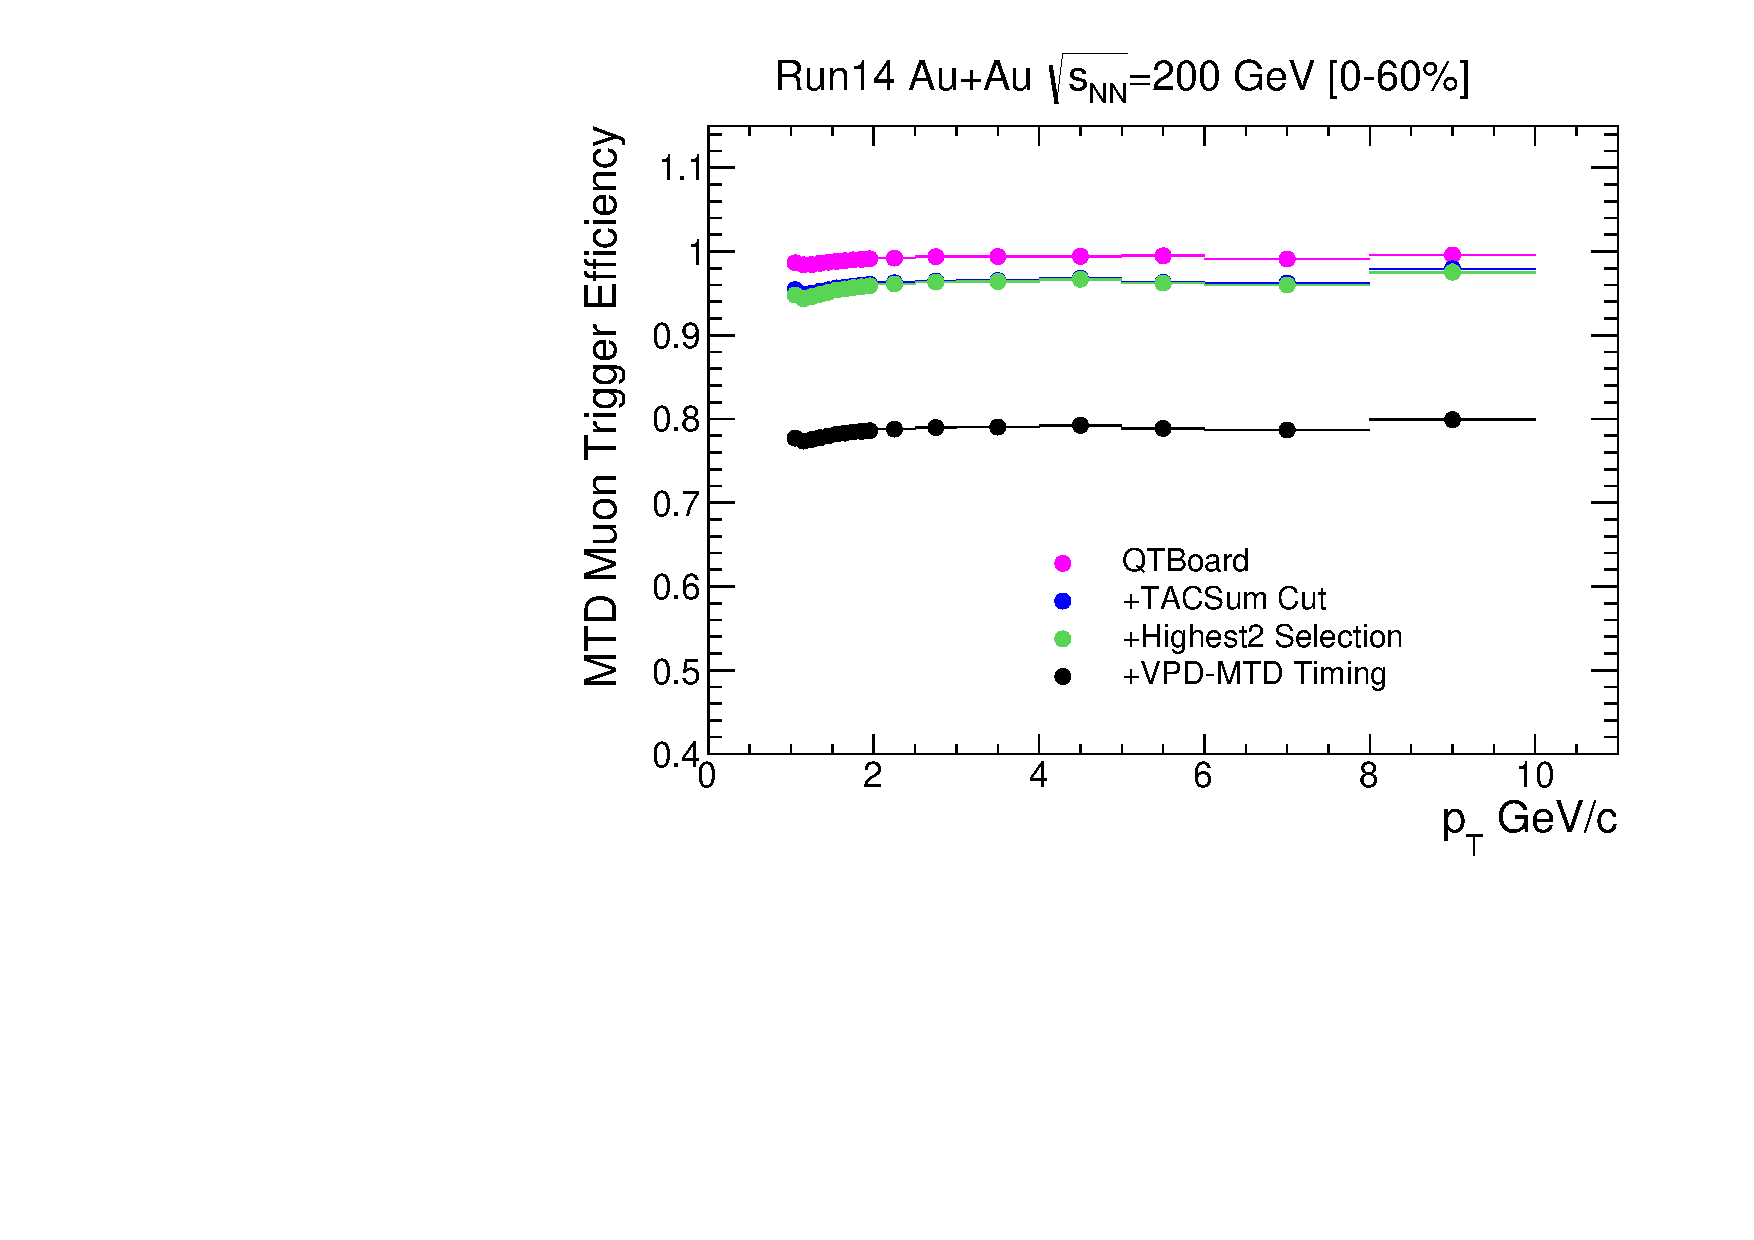
\includegraphics[angle=-90,width=1.0\textwidth]{mtd/MTDTriggerEfficiency.pdf}
\caption{The MTD muon trigger efficiency as a function of $p_{T}$ for the Run14 Au + Au at $\sqrt{s_{NN}}$ = 200 GeV (Centrality: 0-60\%). The muon trigger efficiency including the contribution of both trigger electronics and algorithm is around 78\%.\label{muontrgeff}}
\end{minipage}
\hfill
\begin{minipage}[htbp]{0.48\linewidth}
\centering
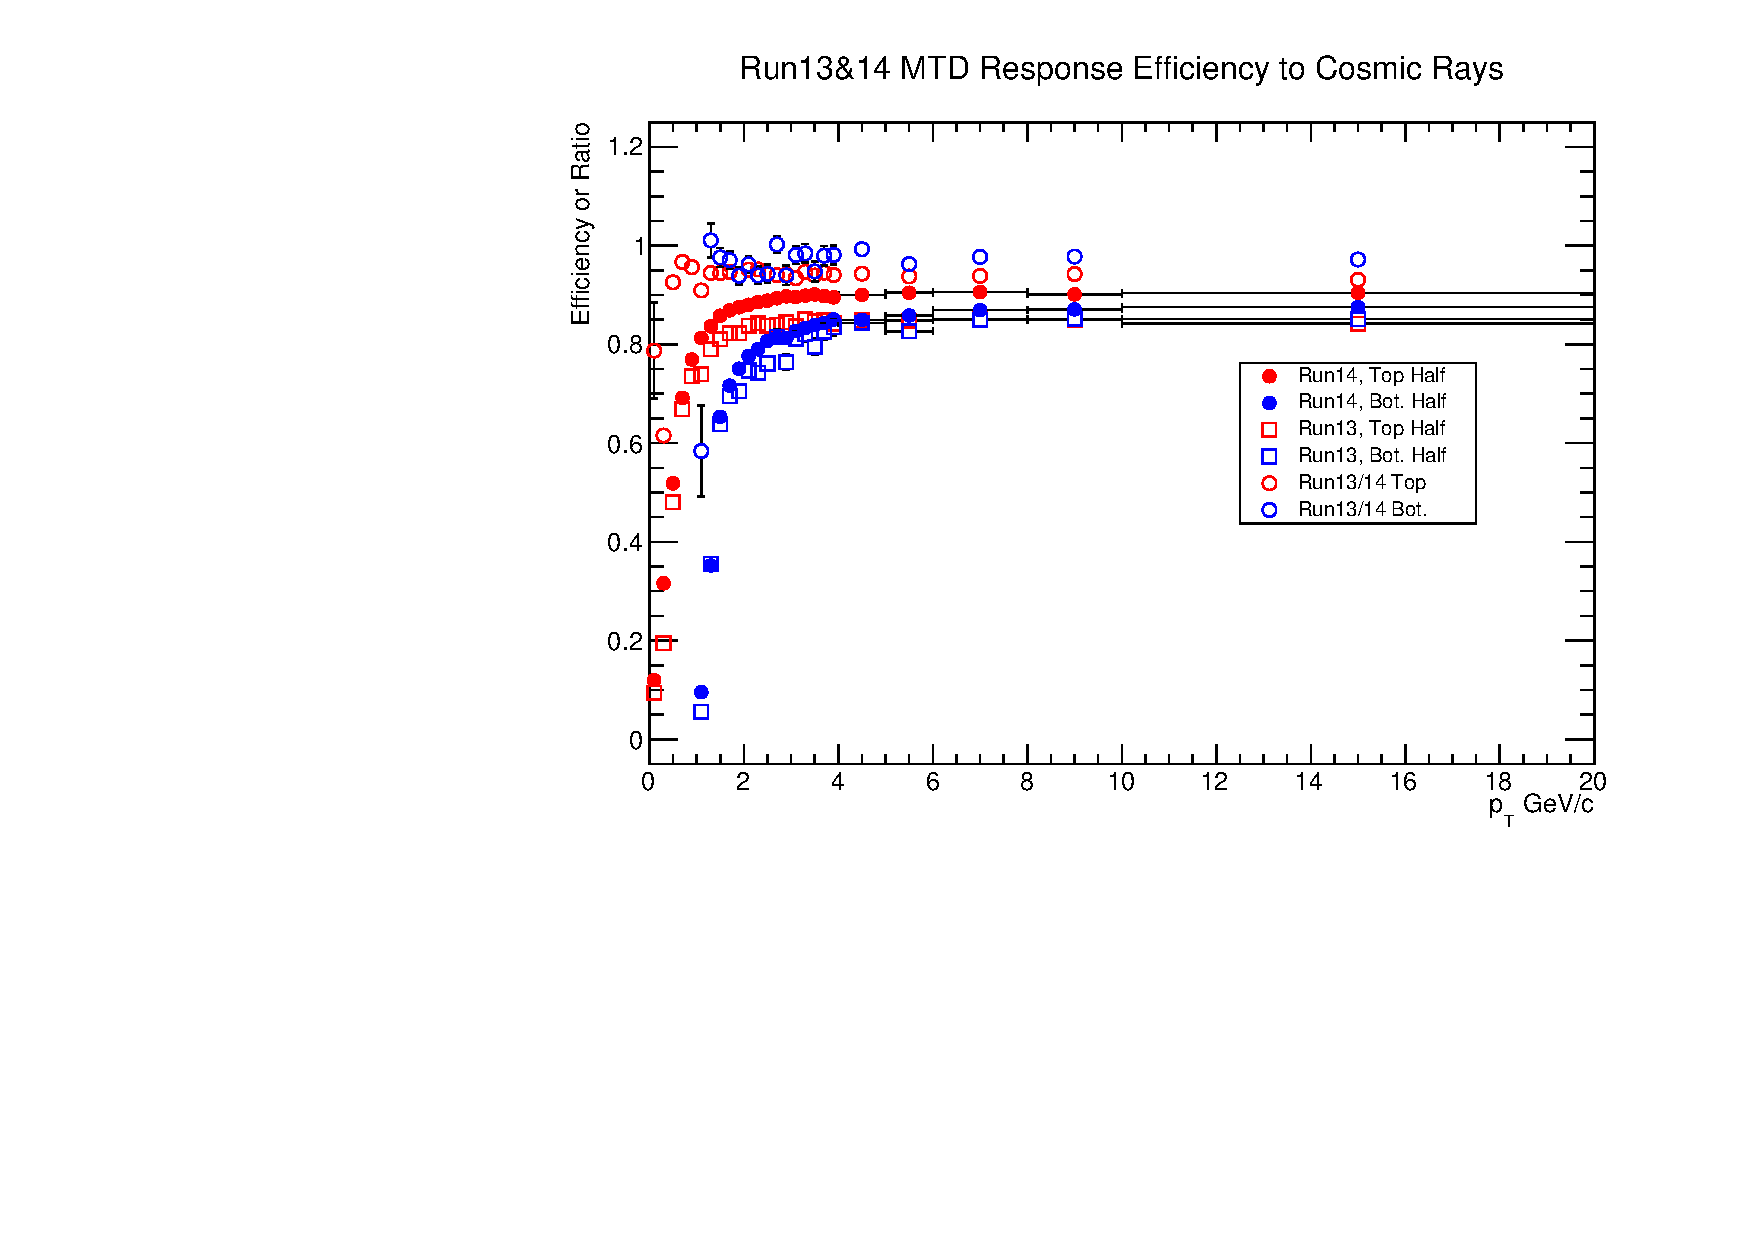
\includegraphics[angle=-90,width=1.0\textwidth]{mtd/MTDResponseEff.pdf} 
\caption{The MTD response efficiency as a function of muon $p_{T}$ for Run13 and Run14. The dots are Run14 response efficiency. The open squares are Run13 response efficiency. The circles are the response ratio between Run13 and Run14.\label{mtdresponseeff}}
\end{minipage}
\end{figure}

\begin{figure}[htbp]
\centering
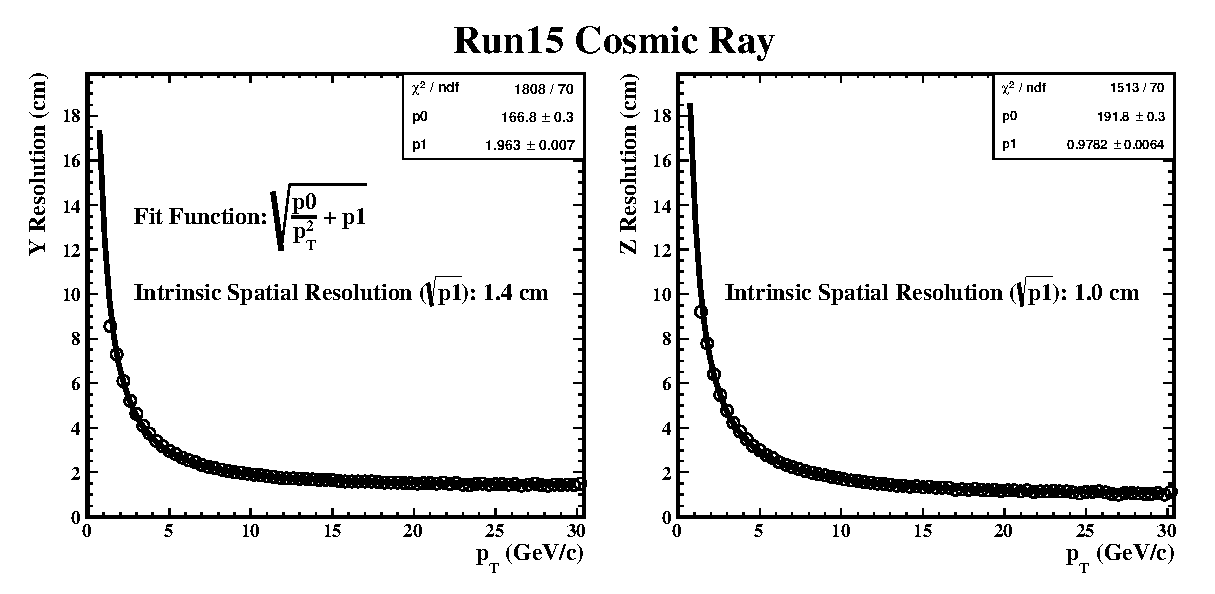
\includegraphics[keepaspectratio,width=1\textwidth]{mtd/posRes.eps}
\figcaption{The intrinsic spatial resolutions of the MTD along $y$ (left panel) and $z$ (right panel) direction as a function of $p_{T}$.}
 \label{posres}
\end{figure}

\begin{figure}[htbp]
\centering
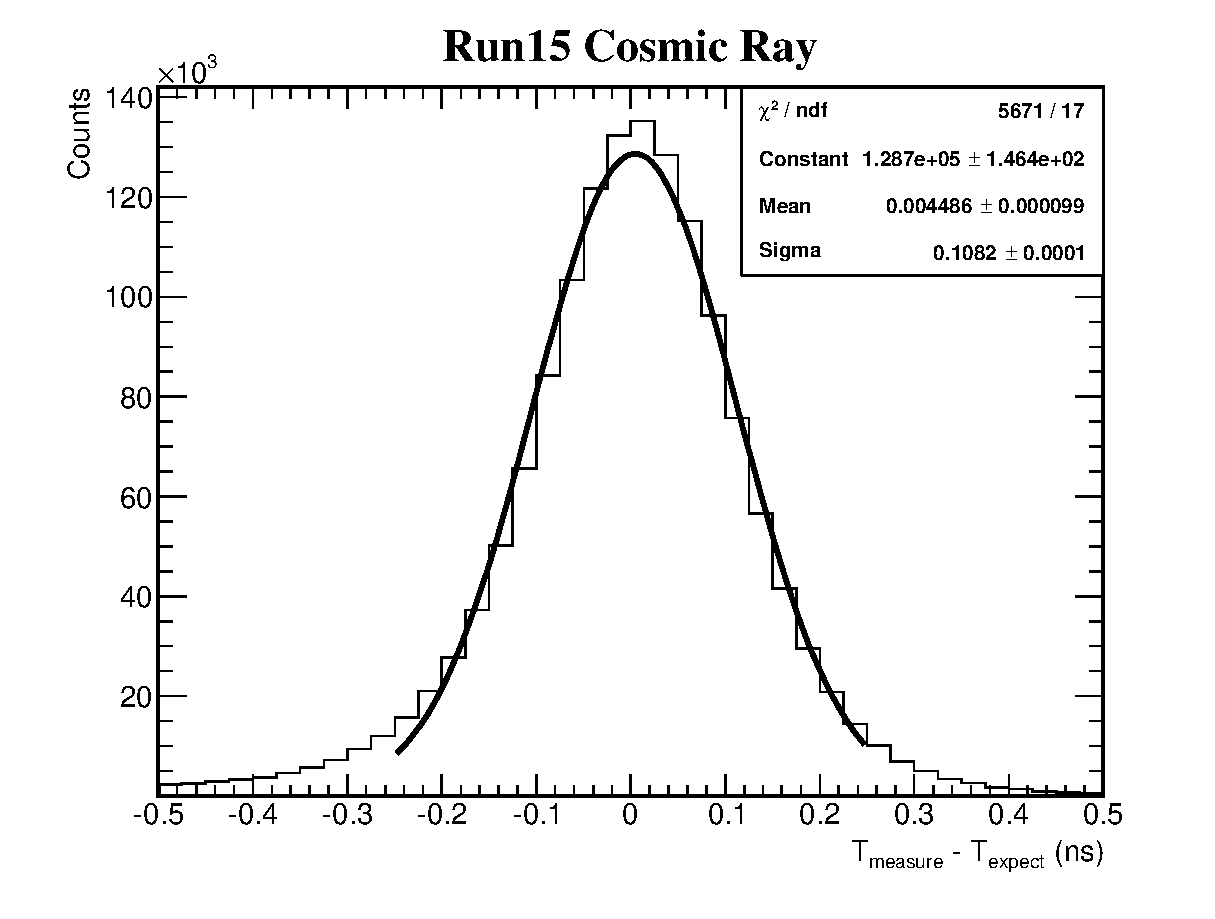
\includegraphics[keepaspectratio,width=0.6\textwidth]{mtd/timeRes.eps}
\figcaption{The overall time resolutions of the MTD (including the starting time contribution, provided by the TOF) after T$_{0}$ and slewing correction.}
 \label{timeRes}
\end{figure}

\section{MTD Performance and Physics Results}
The performance of the MTD system is studied through cosmic ray muons which allow to calibrate the detectors and measure their response efficiency, timing, and spatial resolution due to their very small multiple scattering effect in the detector material. The MTD response efficiency, including both of intrinsic and readout electronics response, can be obtained through calculating the ratio between tracks matched with MTD and tracks projected to MTD. Figure~\ref{mtdresponseeff} shows the MTD response efficiency for Run13 and Run14. The response efficiency trends as a function of $p_{T}$ for Run13 and Run14 are similar. The MTD response efficiency of Run13 is $\sim$85\% for both top half and bottom half while that of Run14 is $\sim$90\%, $\sim$85\% for top half and bottom half, respectively. The top half MTD response efficiency of Run13 is lower than that of Run14, due to electronics damage caused by an unexpected beam loss named ``blue abort kicker prefire''. The $p_{T}$ shift of the MTD response efficiency curves between top half and bottom half is because the cosmic ray muons pass through the magnetic steel firstly and lose energy before they are measured by the TPC. Thus $p_{T}$ measured by the TPC is smaller than the real $p_{T}$ in top half. The spatial resolution, in the $z$ direction (along the readout strips or beam axis direction) and the azimuthal direction ($\phi$ direction, perpendicular to the strips, also called $y$ direction with respect to the MTD module) , of the MTD is measured using the distance between the measured hit position and the track extrapolated position. Figure~\ref{posres} shows the dependence of the spatial resolution along the $y$ direction (left panel, $\Delta$y = R$\times$$\Delta\phi$) and $z$ direction (right panel) as a function of the muon transverse momentum. These data were fit with a function ($\sqrt{(p0/p_{T}^{2}) + p1}$) driven by the expectation for the contribution to the measured resolutions from multiple scattering in the detector materials. The intrinsic spatial resolution is then given by $\sqrt{p1}$. According to Fig.~\ref{posres}, the intrinsic spatial resolutions of the MTD along $y$ and $z$ direction are 1.4 and 1.0 cm, respectively. The time resolution of the MTD system can be measured via the time difference between the measured flight time from the TOF to the MTD and expected time using track extrapolation. After T$_{0}$ and slewing correction, an overall time resolution of 108 ps can be achieved, as shown in Fig.~\ref{timeRes}. The whole procedure and details are described in~\cite{MTDcalib}. The overall time resolution shown in Fig.~\ref{timeRes} includes the contributions from the starting time (56 - 65 ps, $\sigma_{TOF}$/$\sqrt{2}$) and the multiple scattering ($\sim$25 ps for 6 GeV/$c$ muons). The muon can be thus identified in the heavy-ion collisions via precise timing and modest position information.


\begin{figure}[htbp]
\begin{minipage}[htbp]{0.48\linewidth}
\centering
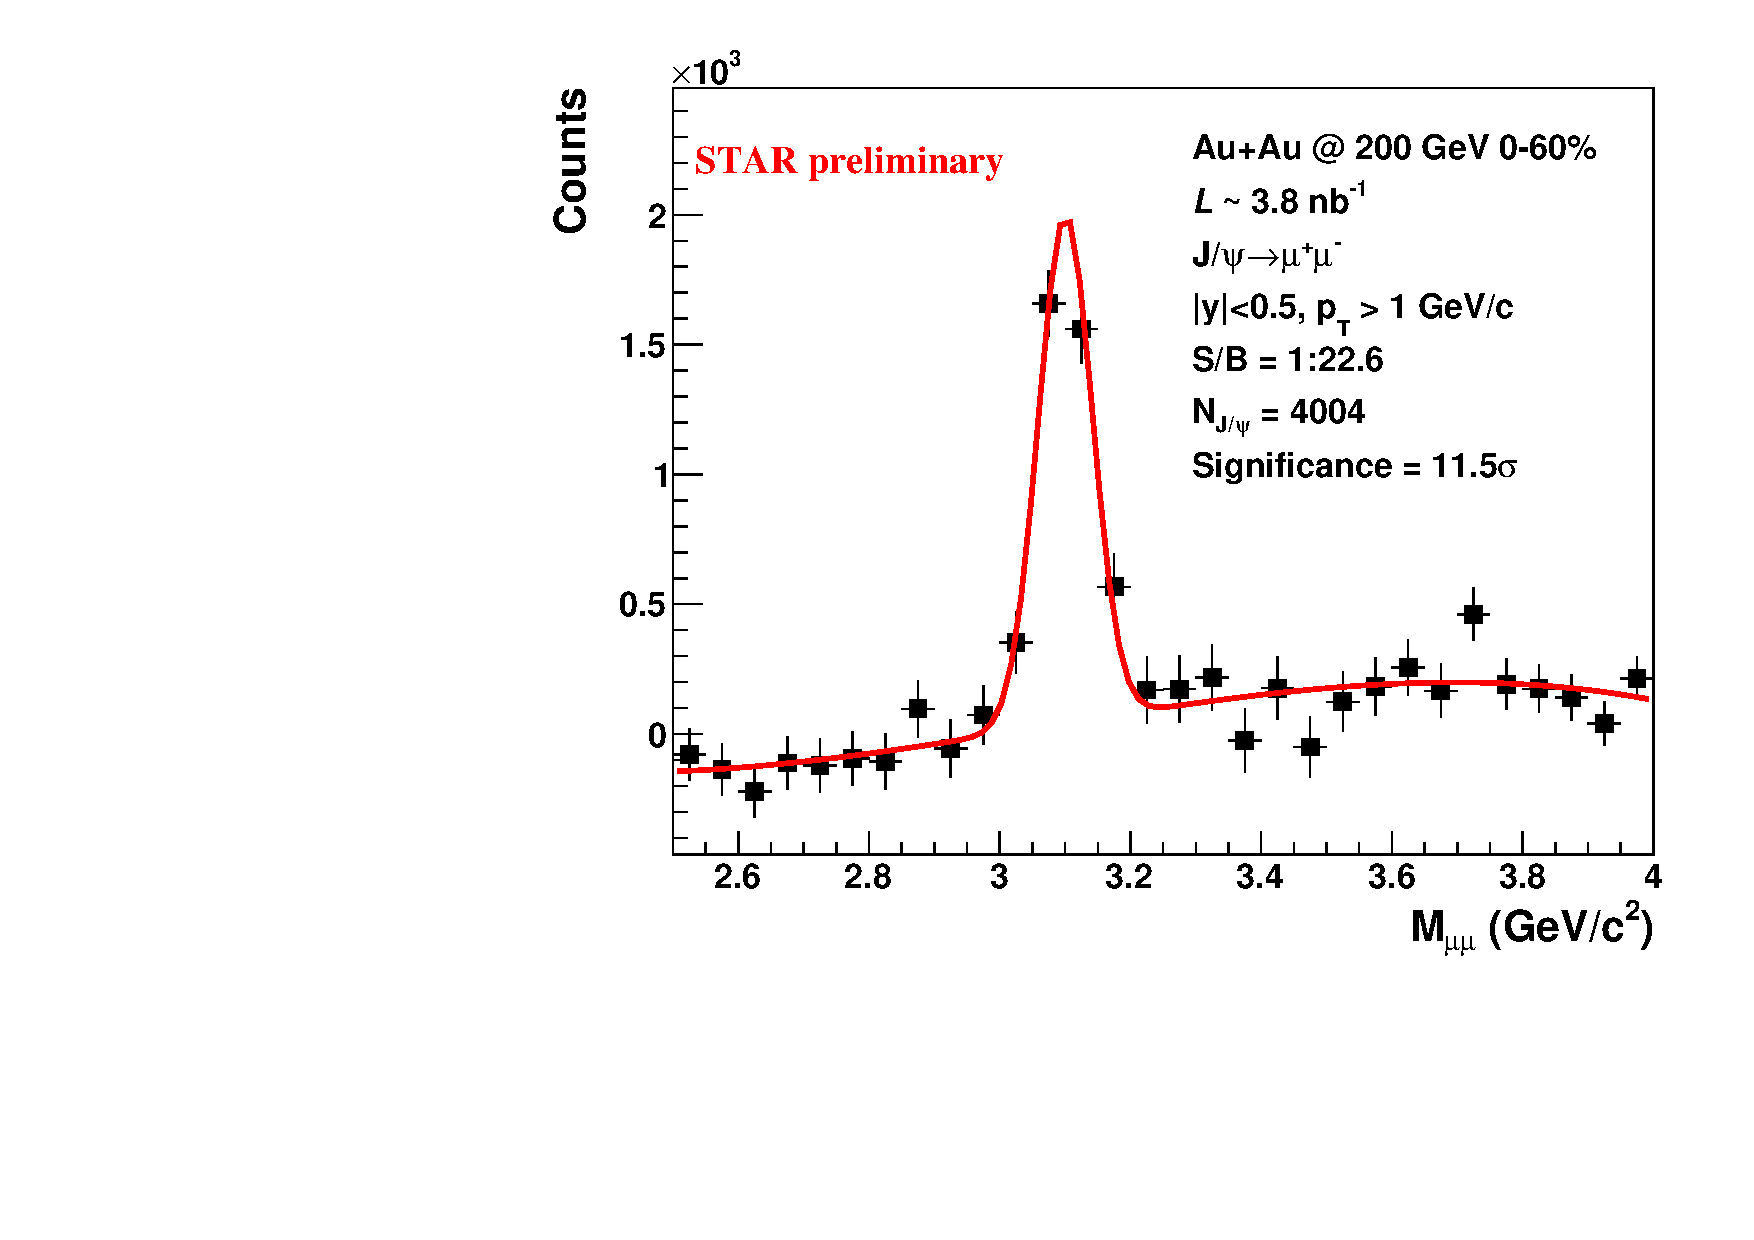
\includegraphics[angle=-90,width=1.0\textwidth]{mtd/Run14_JpsiInvMass.pdf}
\caption{Invariant mass distribution of unlike-sign muon pairs after subtracting mixed-event background. A Gaussian + Pol3 fit to the distribution is shown as the red line.\label{jpsiviamumu}}
\end{minipage}
\hfill
\begin{minipage}[htbp]{0.48\linewidth}
\centering
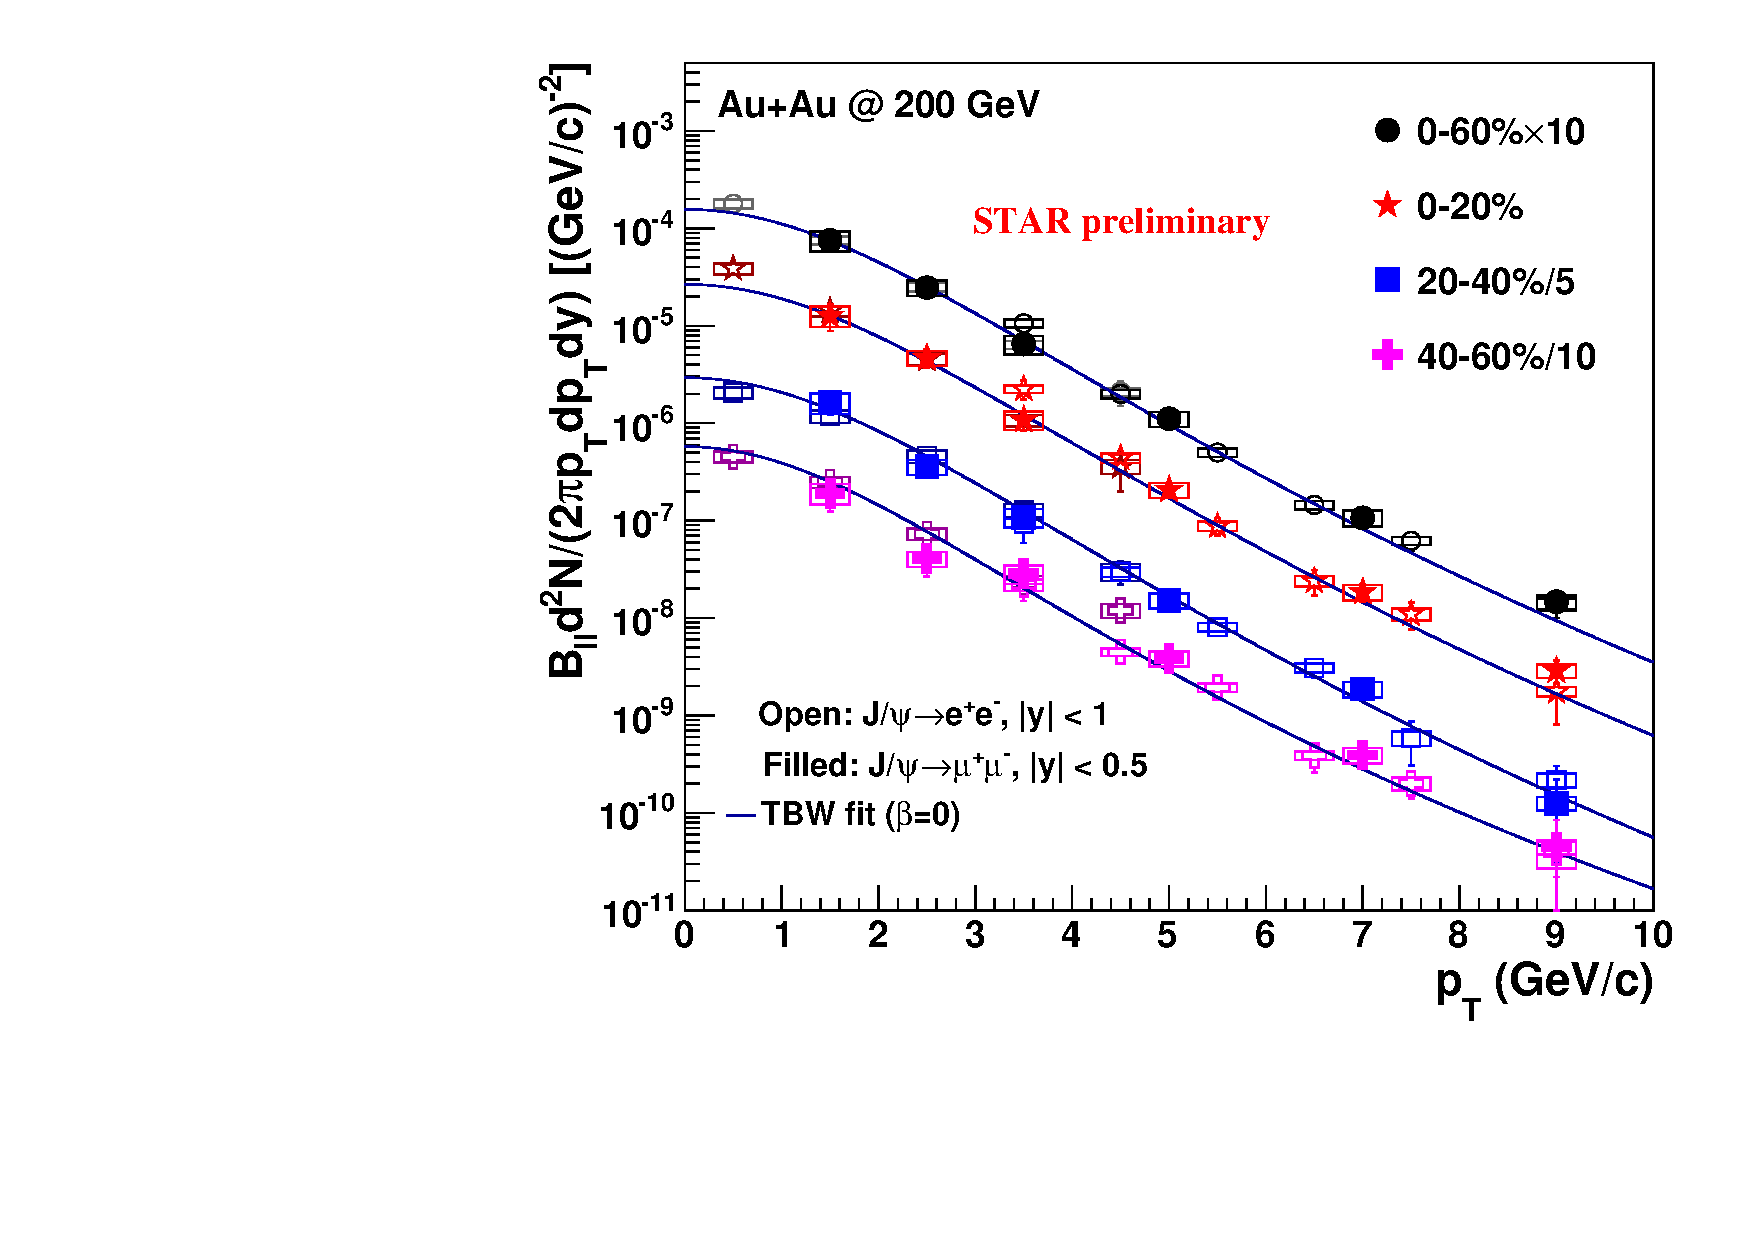
\includegraphics[angle=-90,width=1.0\textwidth]{mtd/Run14_JpsiInvYield_vs_pub.pdf} 
\caption{Invariant yield of inclusive J/$\psi$ vs. $p_{T}$ in four centralities bins (solid markers), with comparison to the published di-electron results (open markers)~\cite{JpsiViaee0, JpsiViaee1}. The solid lines are Tsallis Blast-wave fits to the di-electron results.\label{jpsiyield}}
\end{minipage}
\end{figure}

Lots of physics results from the MTD for Run13 $p$ + $p$ at $\sqrt{s_{NN}}$ = 500 GeV and Run14 Au + Au at $\sqrt{s_{NN}}$ = 200 GeV already came out~\cite{MTDResultpp500, MTDResultAuAu200}. Only part of them are briefly mentioned here. The invariant mass distribution of unlike-sign muon pairs after subtracting the combinatorial background is shown in Fig.~\ref{jpsiviamumu} for Run14 Au + Au at $\sqrt{s_{NN}}$ = 200 GeV. The combinatorial background is estimated via mixed-event technique, namely pairing muons from different events with similar properties. A clear J/$\psi$ peak can be seen with a total of about 4k J/$\psi$ candidates using only $\sim$26.7\% statistics collected in Run14 200 GeV Au + Au collisions. The distribution is fitted by a Gaussian distribution plus a third-order polynomial function (accounting for the residual background). The raw J/$\psi$ is then extracted after subtracting residual background within the mass range of 2.9 - 3.3 GeV/$c^{2}$. After the efficiency losses and detector acceptance are corrected for, the invariant $p_{T}$ spectra of inclusive J/$\psi$ are shown in Fig.~\ref{jpsiyield} for four centrality bins, compared with the published results via di-electron channel~\cite{JpsiViaee0, JpsiViaee1}. The invariant yield spectra measured by di-muon and di-electron channels agree well. $\varUpsilon$ mesons are also reconstructed via the di-muon channel as shown in Fig.~\ref{upsilonviamumu}, where the combinatorial and correlated background are subtracted by using the like-sign same event technique, namely pairing the same charge sign muons into pairs in the same event. A combined fit, constraining the line shape of different $\varUpsilon$ states determined by embedded simulated signals into real data and the shape of residual background ($b\overline{b}$ + Drell-Yan) estimated through PYTHIA simulation, is used to extract the total $\varUpsilon$ yield and the ratio of ($\varUpsilon_{2S}$ + $\varUpsilon_{3S}$)/($\varUpsilon_{1S}$). A total of 50 $\pm$ 22 $\varUpsilon$s are observed and a factor of 6 more statistics is expected combining the rest of 2014 data and the data that will be taken in 2016. Figure~\ref{upsilonproj} shows the projection for the statistical uncertainty on the ratio of ($\varUpsilon_{2S}$ + $\varUpsilon_{3S}$)/($\varUpsilon_{1S}$) using the full statistics of Run14 and Run16 for Au + Au at $\sqrt{s_{NN}}$ = 200 GeV, together with the published results in different collision systems at different energies~\cite{UpsilonWorldwide, UpsilonSTAR, UpsilonCMS}.

\begin{figure}[htbp]
\begin{minipage}[htbp]{0.48\linewidth}
\centering
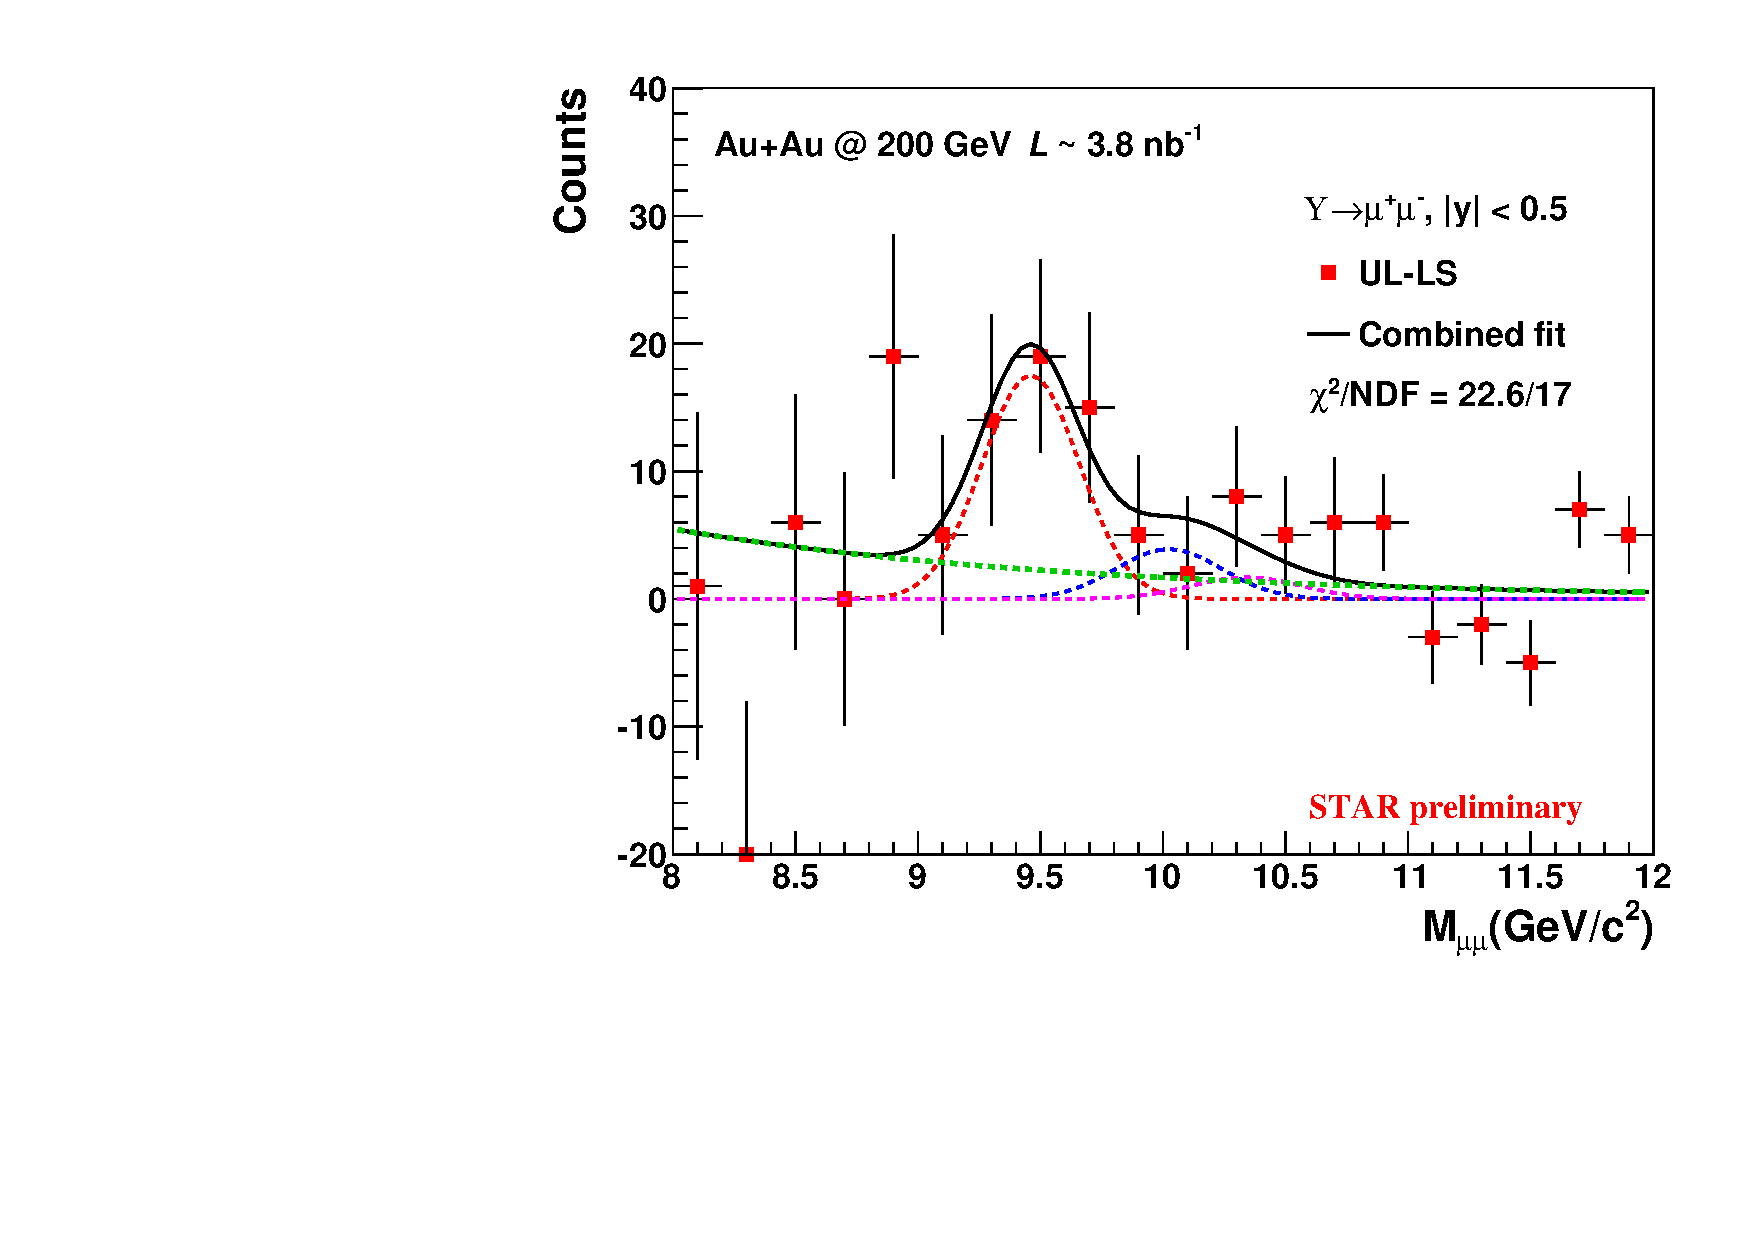
\includegraphics[angle=-90,width=1.0\textwidth]{mtd/Run14_Upsilon.pdf}
\caption{ Invariant mass distribution of unlike-sign dimuon pairs after subtracting the like-sign distribution (red points).
A combined fit of signal and residual background ($b\overline{b}$ + Drell-Yan) is shown as the solid black curve.\label{upsilonviamumu}}
\end{minipage}
\hfill
\begin{minipage}[htbp]{0.48\linewidth}
\centering
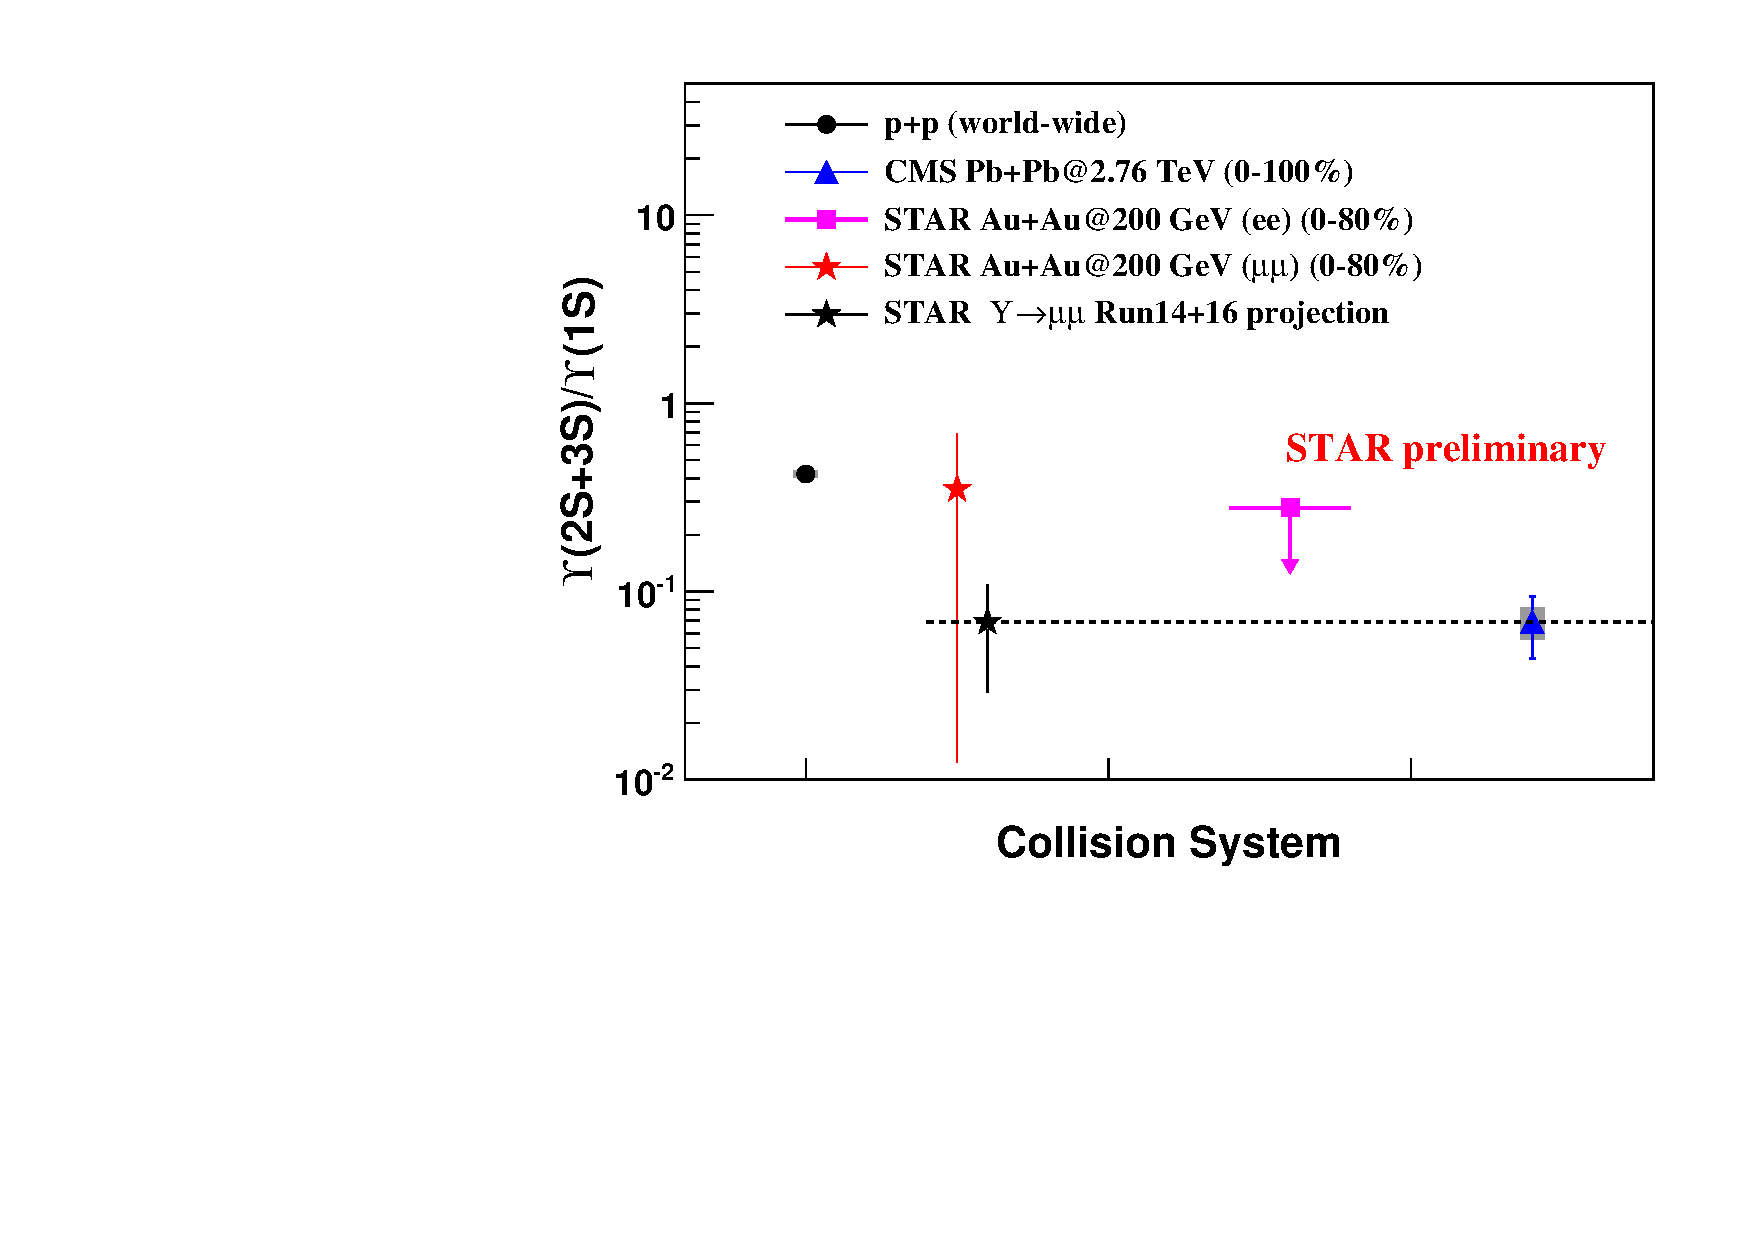
\includegraphics[angle=-90,width=1.0\textwidth]{mtd/Run14_Upsilon_Ratio_log.pdf} 
\caption{The projection of ($\varUpsilon_{2S}$ + $\varUpsilon_{3S}$)/($\varUpsilon_{1S}$) using full statistics of Run14 and Run16 Au+Au data collected by the MTD, together with the published results in different collision systems at different energies~\cite{UpsilonWorldwide, UpsilonSTAR, UpsilonCMS}.\label{upsilonproj}}
\end{minipage}
\end{figure}

We are still investigating the characteristics of hadrons recorded by the MTD and developing a better muon identification method. Once a pure muon sample can be identified, the di-$\mu$ and e-$\mu$ spectra using the full-statistics 200 GeV Au + Au data will be measured, which will provide a direct access to the QGP thermal radiation.

%封面是按照制本厂的要求制作的,其中行宽和行高都是固定的,中文标题最多占两行,英文标题最多占三行。如果您的题目超过了这个限制,请缩减题目长度,不要擅自修改模板中的相关配置参数。

